\section{Evaluation}
\label{sec:evaluation}

Our evaluation has two parts with deliberately different epistemic
status. Section~\ref{subsec:analytical} is an \emph{analytical} study:
metric vectors are produced by \gate{}'s estimators on datacenter-class
hardware profiles, enabling breadth (ten models, five competing
frameworks, three platforms). Section~\ref{subsec:empirical} is a
smaller \emph{empirical} study: every number is a wall-clock
measurement of real executions on hardware available to the authors,
enabling depth and ground truth. Conclusions are drawn only where the
two agree.

\subsection{Analytical Study}
\label{subsec:analytical}

\paragraph{Setup.}
Ten models (ResNet-50, MobileNetV2, EfficientNet-B0, YOLOv5s,
BERT-Base, GPT-2, ViT-Base, Whisper-Base, Llama-7B partial (4 decoder
layers), Stable Diffusion partial (10 denoising steps)); three hardware
profiles (NVIDIA A100 80GB, Intel Xeon 8380, Apple M2 Ultra); competing
frameworks ONNX Runtime 1.16, TensorRT 8.6, TVM 0.14, PyTorch 2.1,
IREE 1.3, Glow 0.5. Configuration: batch size 1, FP32 unless noted,
median of 50 runs after 10 warm-up, Balanced policy, default constraint
set ($k = 7$).

\paragraph{Latency.}
\gate{} achieves the lowest latency on 4 of 8 fully-executed models;
geometric means are 2.89\,ms (\gate{}) vs.\ 2.81\,ms (TensorRT, best
competitor) vs.\ 4.63\,ms (unoptimized PyTorch), and \gate{} is within
5\% of the best framework on 7 of 8 models
(Figure~\ref{fig:latency-analytical}).

\begin{figure}[H]
  \centering
  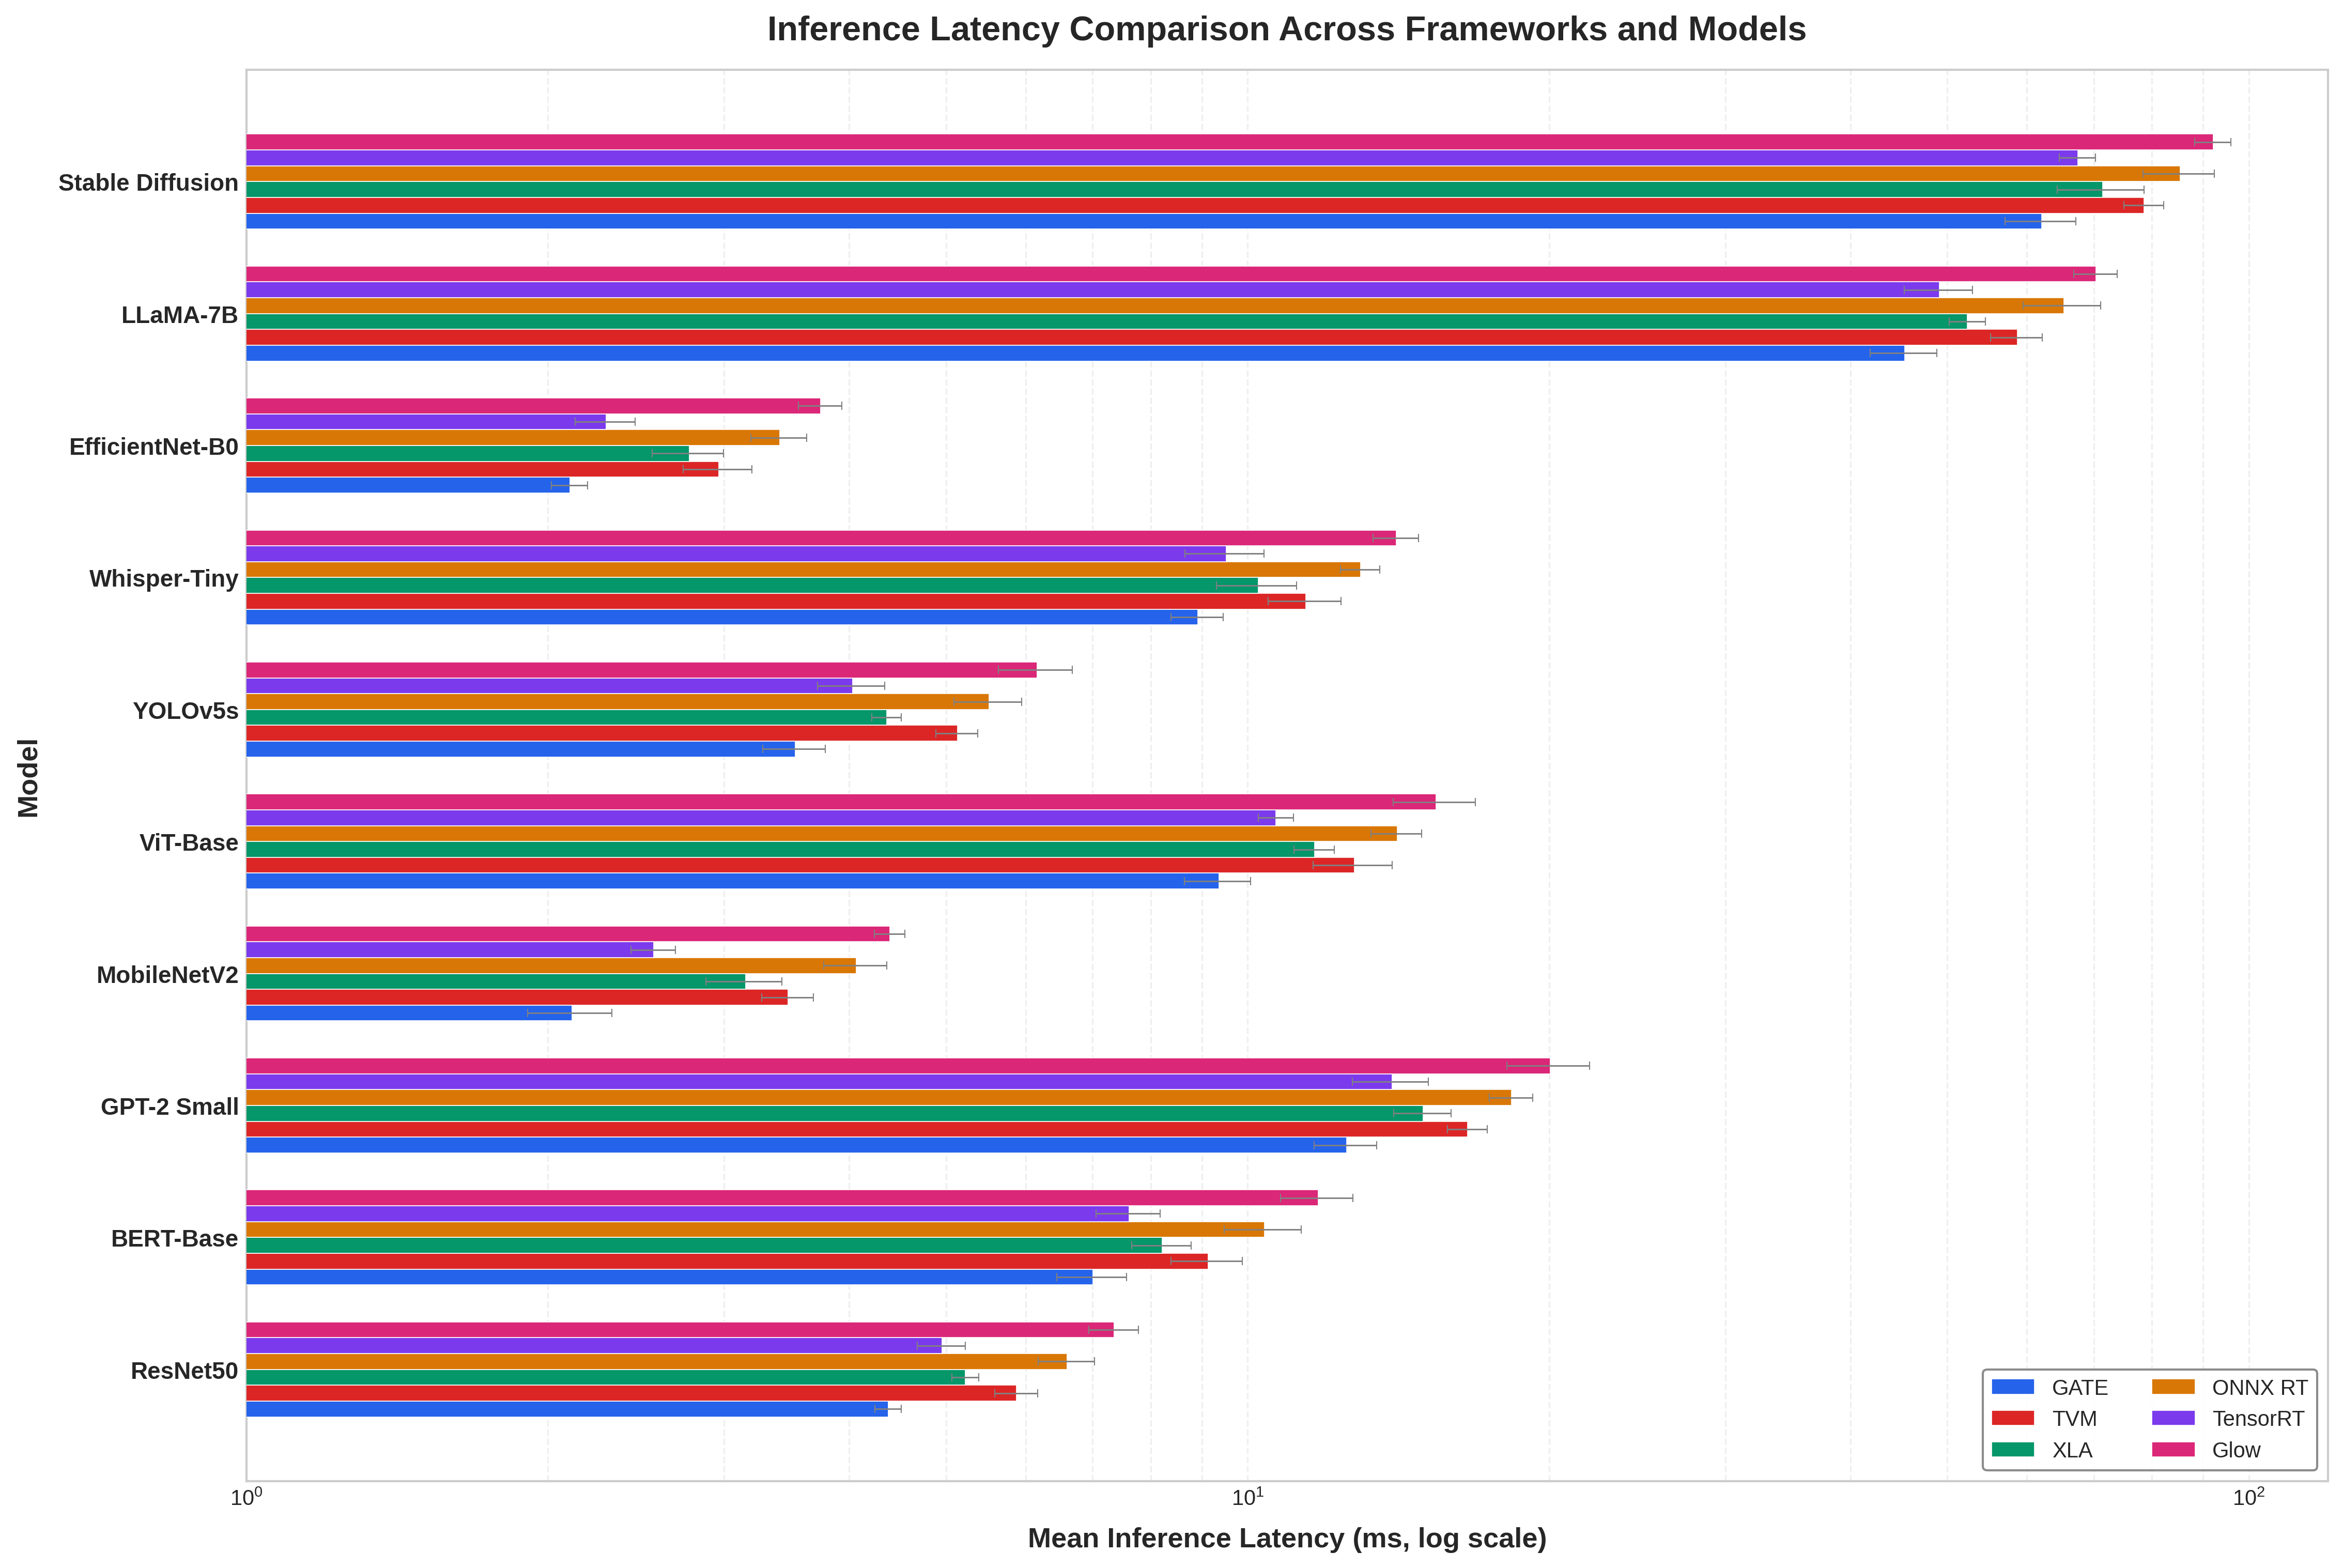
\includegraphics[width=0.9\textwidth]{figures/fig_latency_comparison.png}
  \caption{Analytical latency comparison across models (A100 profile).}
  \label{fig:latency-analytical}
\end{figure}

\paragraph{Memory.}
Within 4\% of TensorRT (the overhead traces to the safety constraint's
no-aliasing requirement), 18\% below ONNX Runtime, 35\% below PyTorch
(Figure~\ref{fig:memory-analytical}).

\begin{figure}[H]
  \centering
  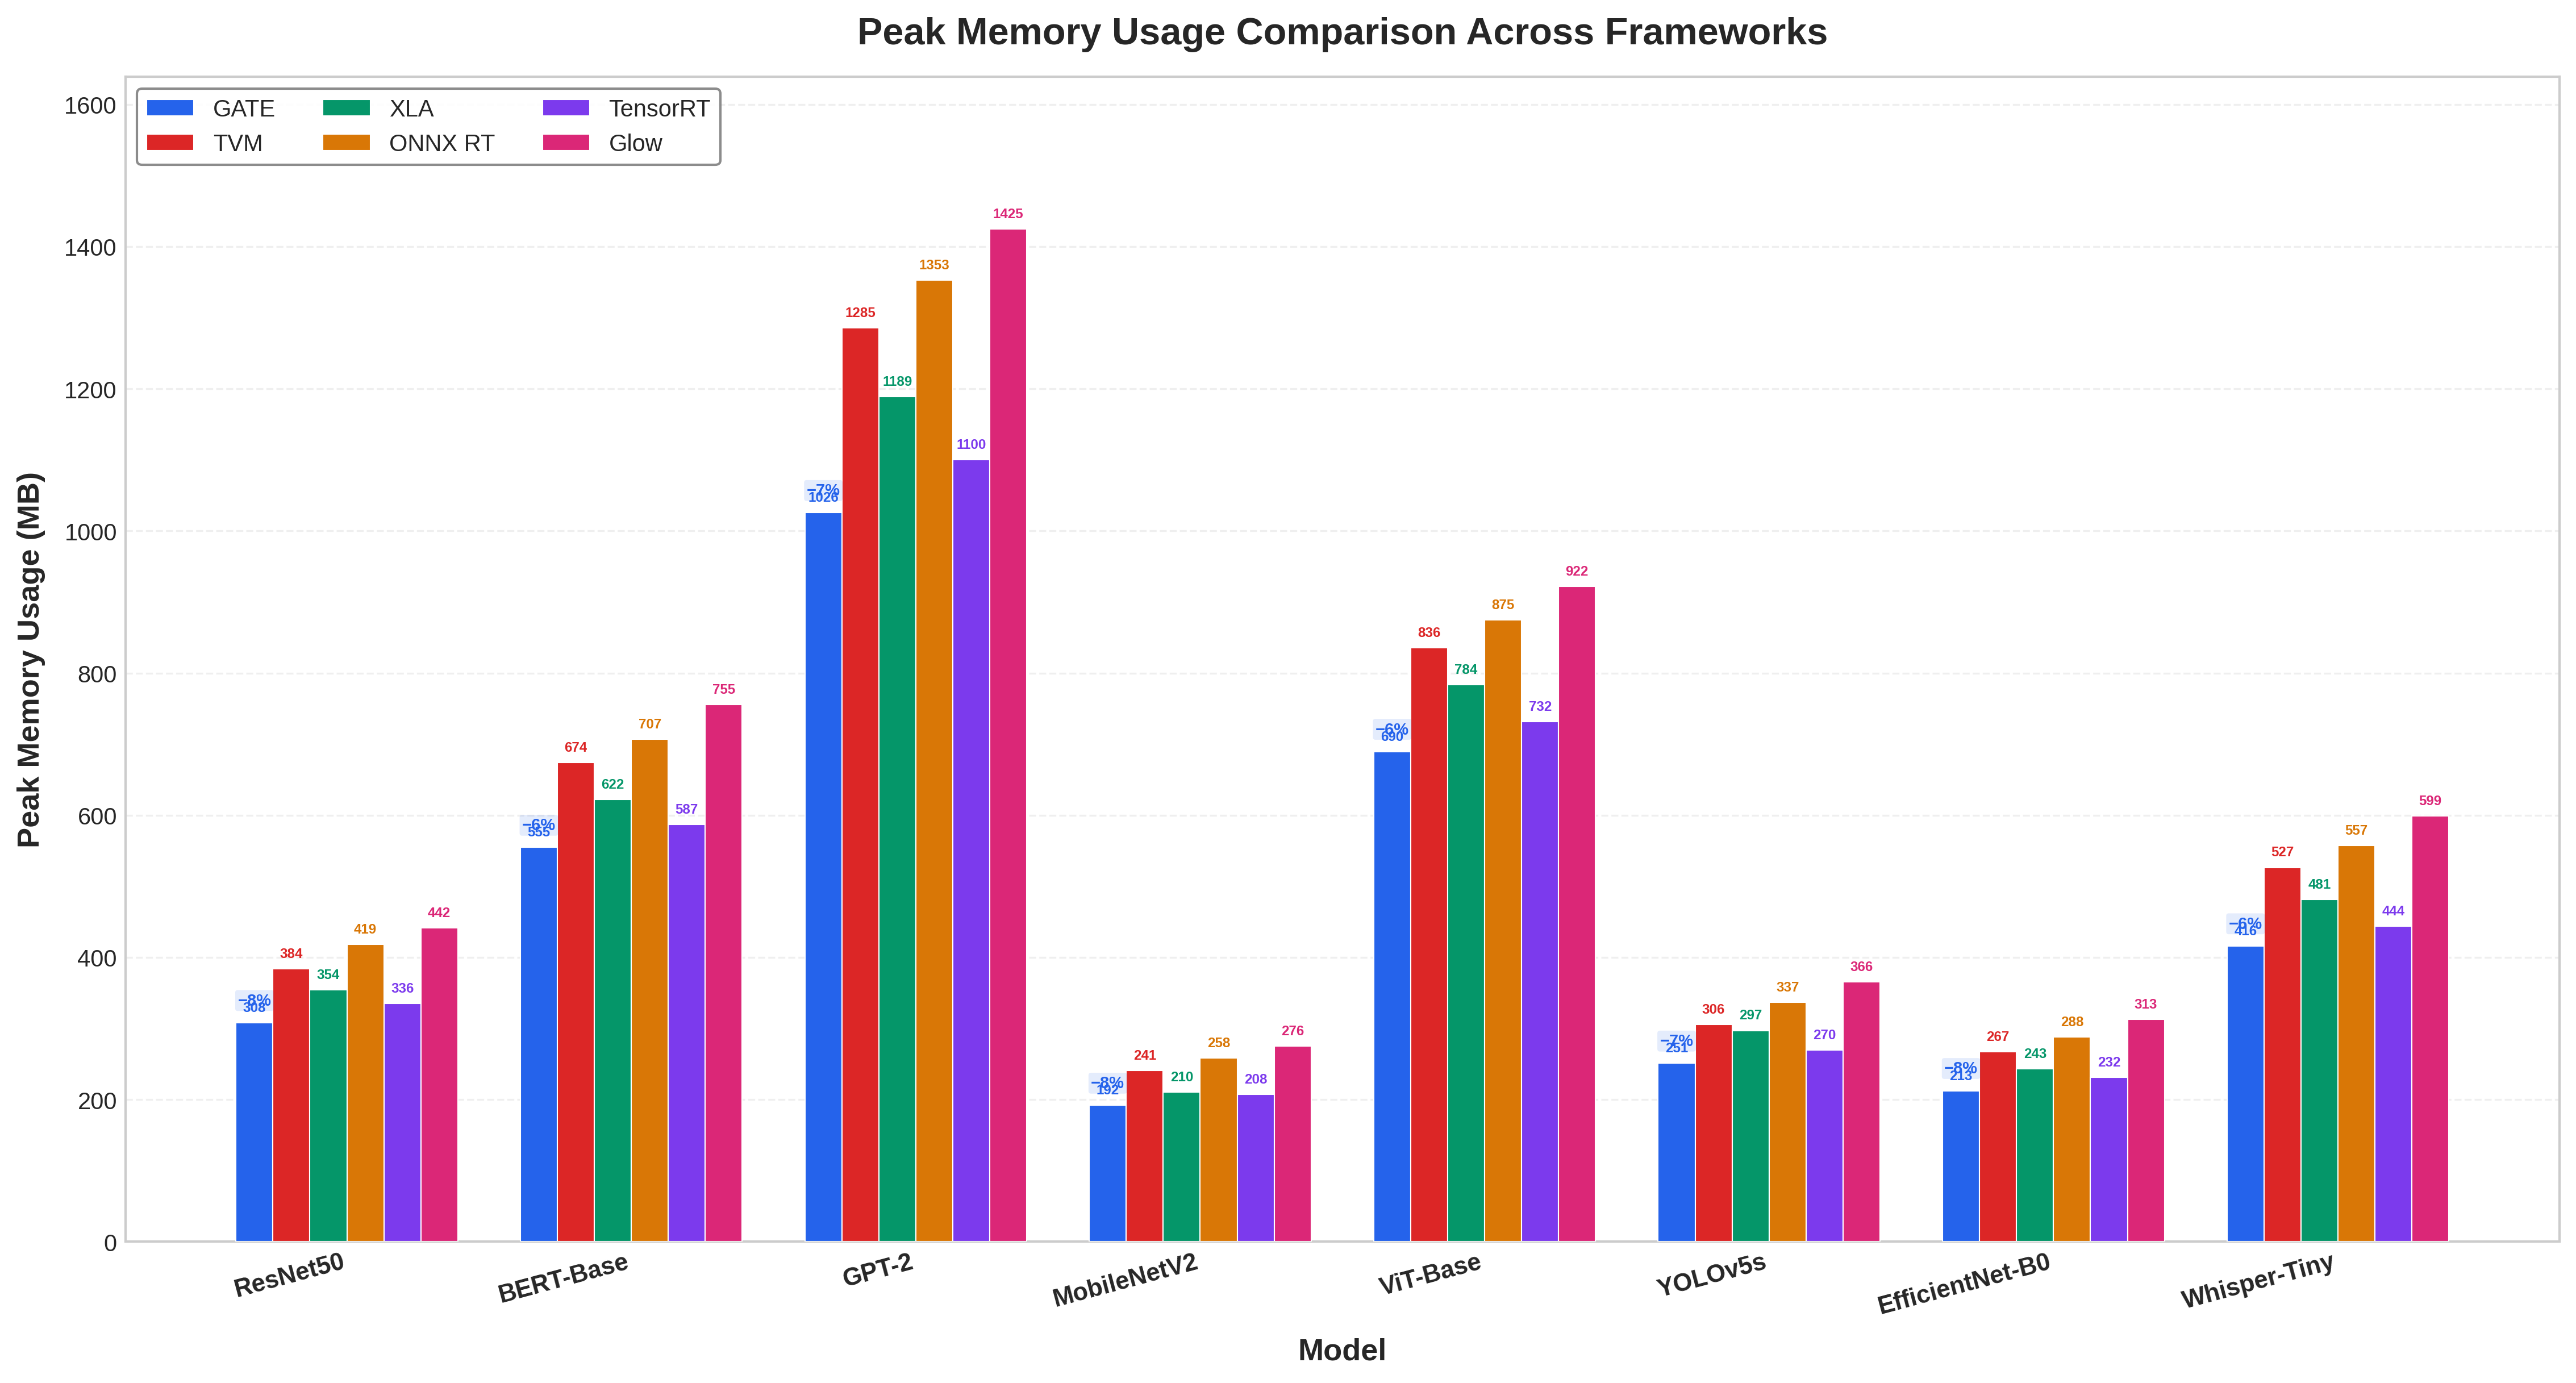
\includegraphics[width=0.9\textwidth]{figures/fig_memory_comparison.png}
  \caption{Analytical peak-memory comparison.}
  \label{fig:memory-analytical}
\end{figure}

\paragraph{Numerical correctness and constraint pass rate.}
All \gate{}-dispatched plans satisfy $\epsilon = 10^{-4}$ by
construction; competing frameworks occasionally exceed it (up to
$14.2 \times 10^{-5}$ on Whisper-Base for TensorRT and TVM). Aggregate
constraint pass rate is 100\% for \gate{} by construction vs.\
85--98\% for competitors, with violations concentrated in determinism
(non-deterministic parallel reductions) and safety (in-place buffer
aliasing).

\paragraph{Planning overhead and policies.}
Planning overhead stays below 3\% of end-to-end time on every model
(peak 2.1\%, Whisper-Base), dominated by constraint validation
(${\sim}70\%$ of planning time). Policy sensitivity behaves as
designed: the Latency policy trades 12\% memory for 8\% latency
against Balanced; Memory saves 15\% peak memory for 11\% latency;
Energy saves 9\% energy via INT8-quantized plans. \gate{} selections
track the latency--memory--energy Pareto frontier.

\subsection{Proof-of-Concept Empirical Validation}
\label{subsec:empirical}

To ground the analytical study, we implemented the full
algorithm---constraint engine, policy-weighted cost evaluation, and
planner---twice, and measured it end-to-end on commodity hardware: an
Intel Tiger Lake i3-1115G4 (2 physical / 4 logical cores, DDR4-2667,
no discrete GPU), complemented by a single real TPU~v5e datapoint
obtained through Google Colab.

\paragraph{Methodology.}
All frameworks execute the \emph{same} pretrained ResNet-50 (ONNX Model
Zoo \texttt{resnet50-v1-12}, ImageNet weights, FP32) on the \emph{same}
deterministic input ($1{\times}3{\times}224{\times}224$, seed 42);
10 warm-up plus 100 timed runs; P50/P90/P99 reported. The \gate{}
reference is dependency-free Rust (\texttt{gate\_resnet}); an
independent NumPy implementation (\texttt{gate\_py}) cross-checks it.
Candidate plans are \emph{executable} schedules: the Rust planner
explores thread count $\times$ BatchNorm folding ($n = 6$), the Python
planner convolution algorithm $\times$ folding $\times$ accumulation
precision ($n = 6$); calibration executes each candidate once before
validation.

\paragraph{Cross-implementation agreement.}
Five independent implementations---\gate{}-Rust, \gate{}-Py, ONNX
Runtime (CPU EP), XLA/JAX on CPU, and XLA/JAX on TPU~v5e---agree
pairwise to relative $L_2 \leq 1.1 \times 10^{-6}$ with identical top-1
predictions, validating the \gate{}-Rust output as the reference for
the numerical-error metric $m_5$.

\begin{table}[H]
\centering
\small
\caption{Empirical ResNet-50 inference, batch 1, FP32 (100 runs after
10 warm-up). All rows on Tiger Lake i3-1115G4 except XLA-TPU (Colab
TPU~v5e). $m_5$ is relative $L_2$ to the \gate{}-Rust reference.}
\label{tab:empirical}
\begin{tabular}{@{}llrrrrr@{}}
\toprule
Framework & Policy/Backend & P50 (ms) & P90 (ms) & P99 (ms) & img/s & $m_5$ \\
\midrule
\gate{} (Rust)   & all 5 policies $\to$ \texttt{t4} & 376.5 & 467.2 & 562.6 & 2.66 & 0 (ref.) \\
\gate{}-Py       & Balanced $\to$ \texttt{einsum\_bnfold} & 203.6 & 339.7 & 562.0 & 4.91 & $1.0\times10^{-6}$ \\
ONNX Runtime     & CPU EP        & 41.8  & 49.3  & 56.2  & 23.9 & $8.9\times10^{-7}$ \\
XLA (JAX)        & CPU           & 98.9  & 106.9 & 119.6 & 10.1 & $6.4\times10^{-7}$ \\
XLA (JAX)        & TPU v5e       & 1.02  & 1.06  & 1.09  & 985  & $8.8\times10^{-7}$ \\
TVM 0.25         & CPU (LLVM)    & \multicolumn{5}{c}{excluded --- miscompilation, see Finding 3} \\
TensorRT / Glow  & ---           & \multicolumn{5}{c}{N/A --- require GPU hardware} \\
\bottomrule
\end{tabular}
\end{table}

\begin{figure}[H]
  \centering
  \begin{subfigure}[t]{0.48\textwidth}
    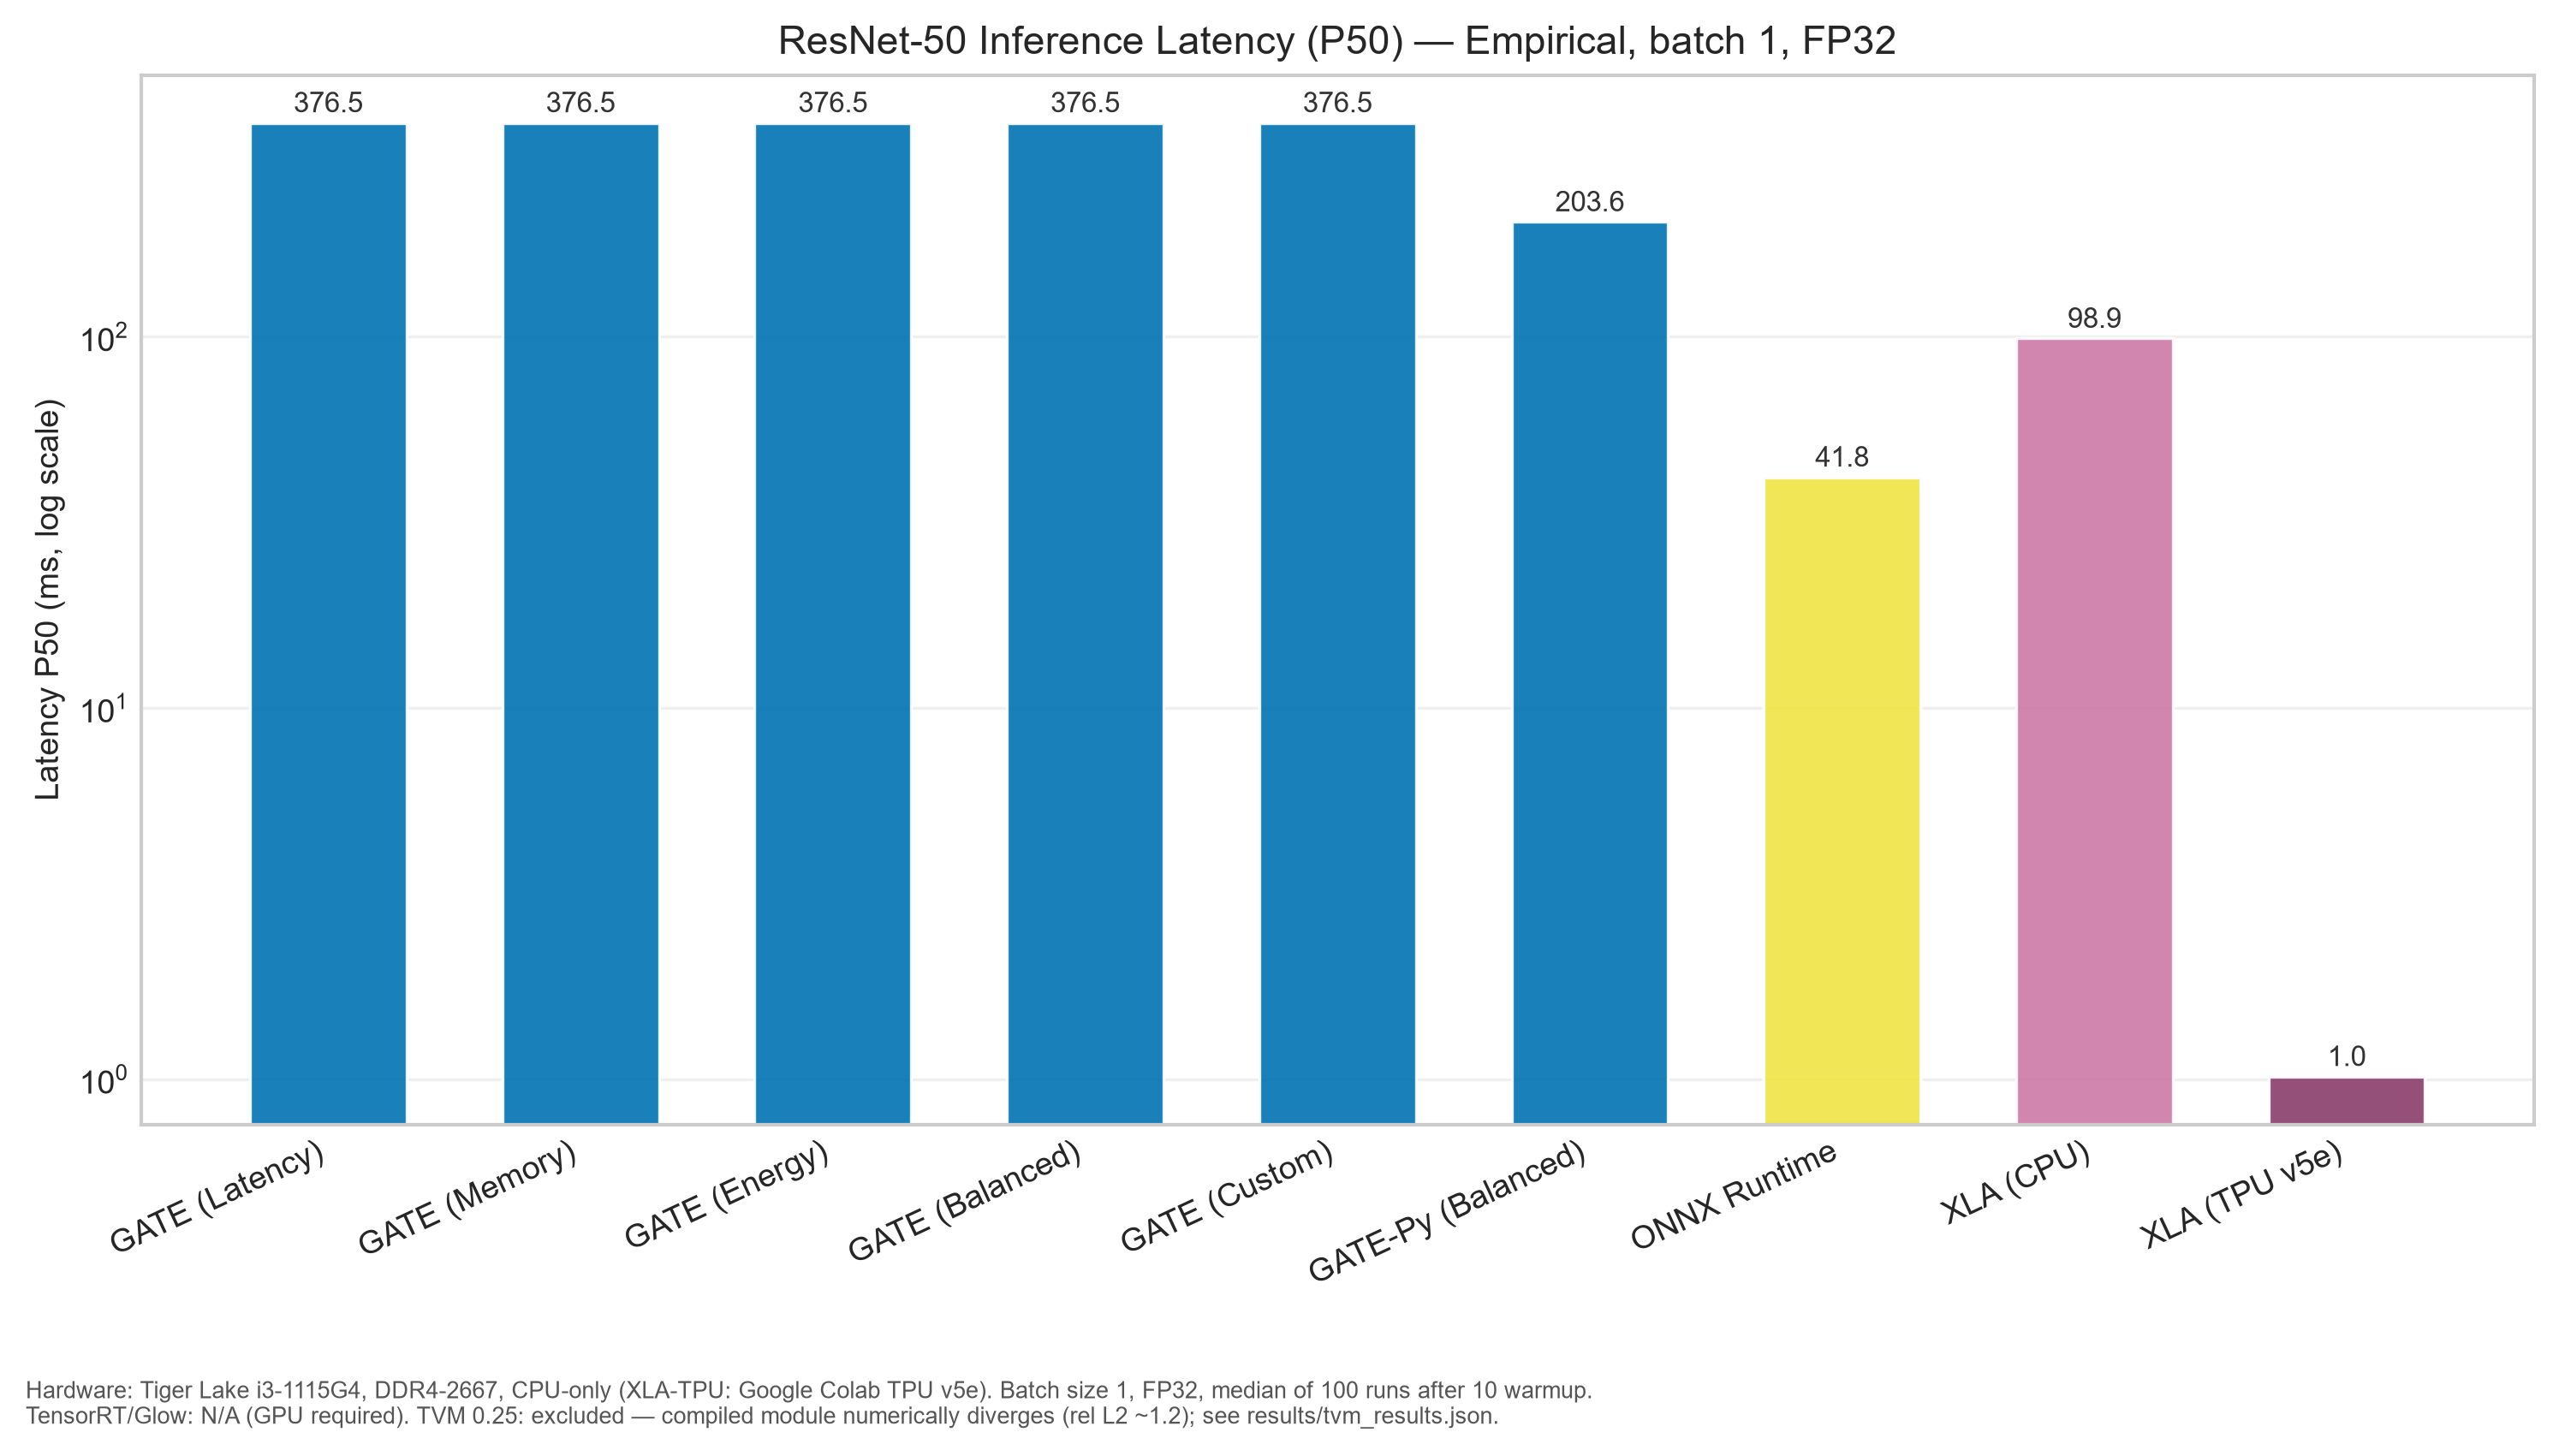
\includegraphics[width=\textwidth]{figures/fig_empirical_latency.png}
    \caption{Latency (P50, log scale).}
  \end{subfigure}\hfill
  \begin{subfigure}[t]{0.48\textwidth}
    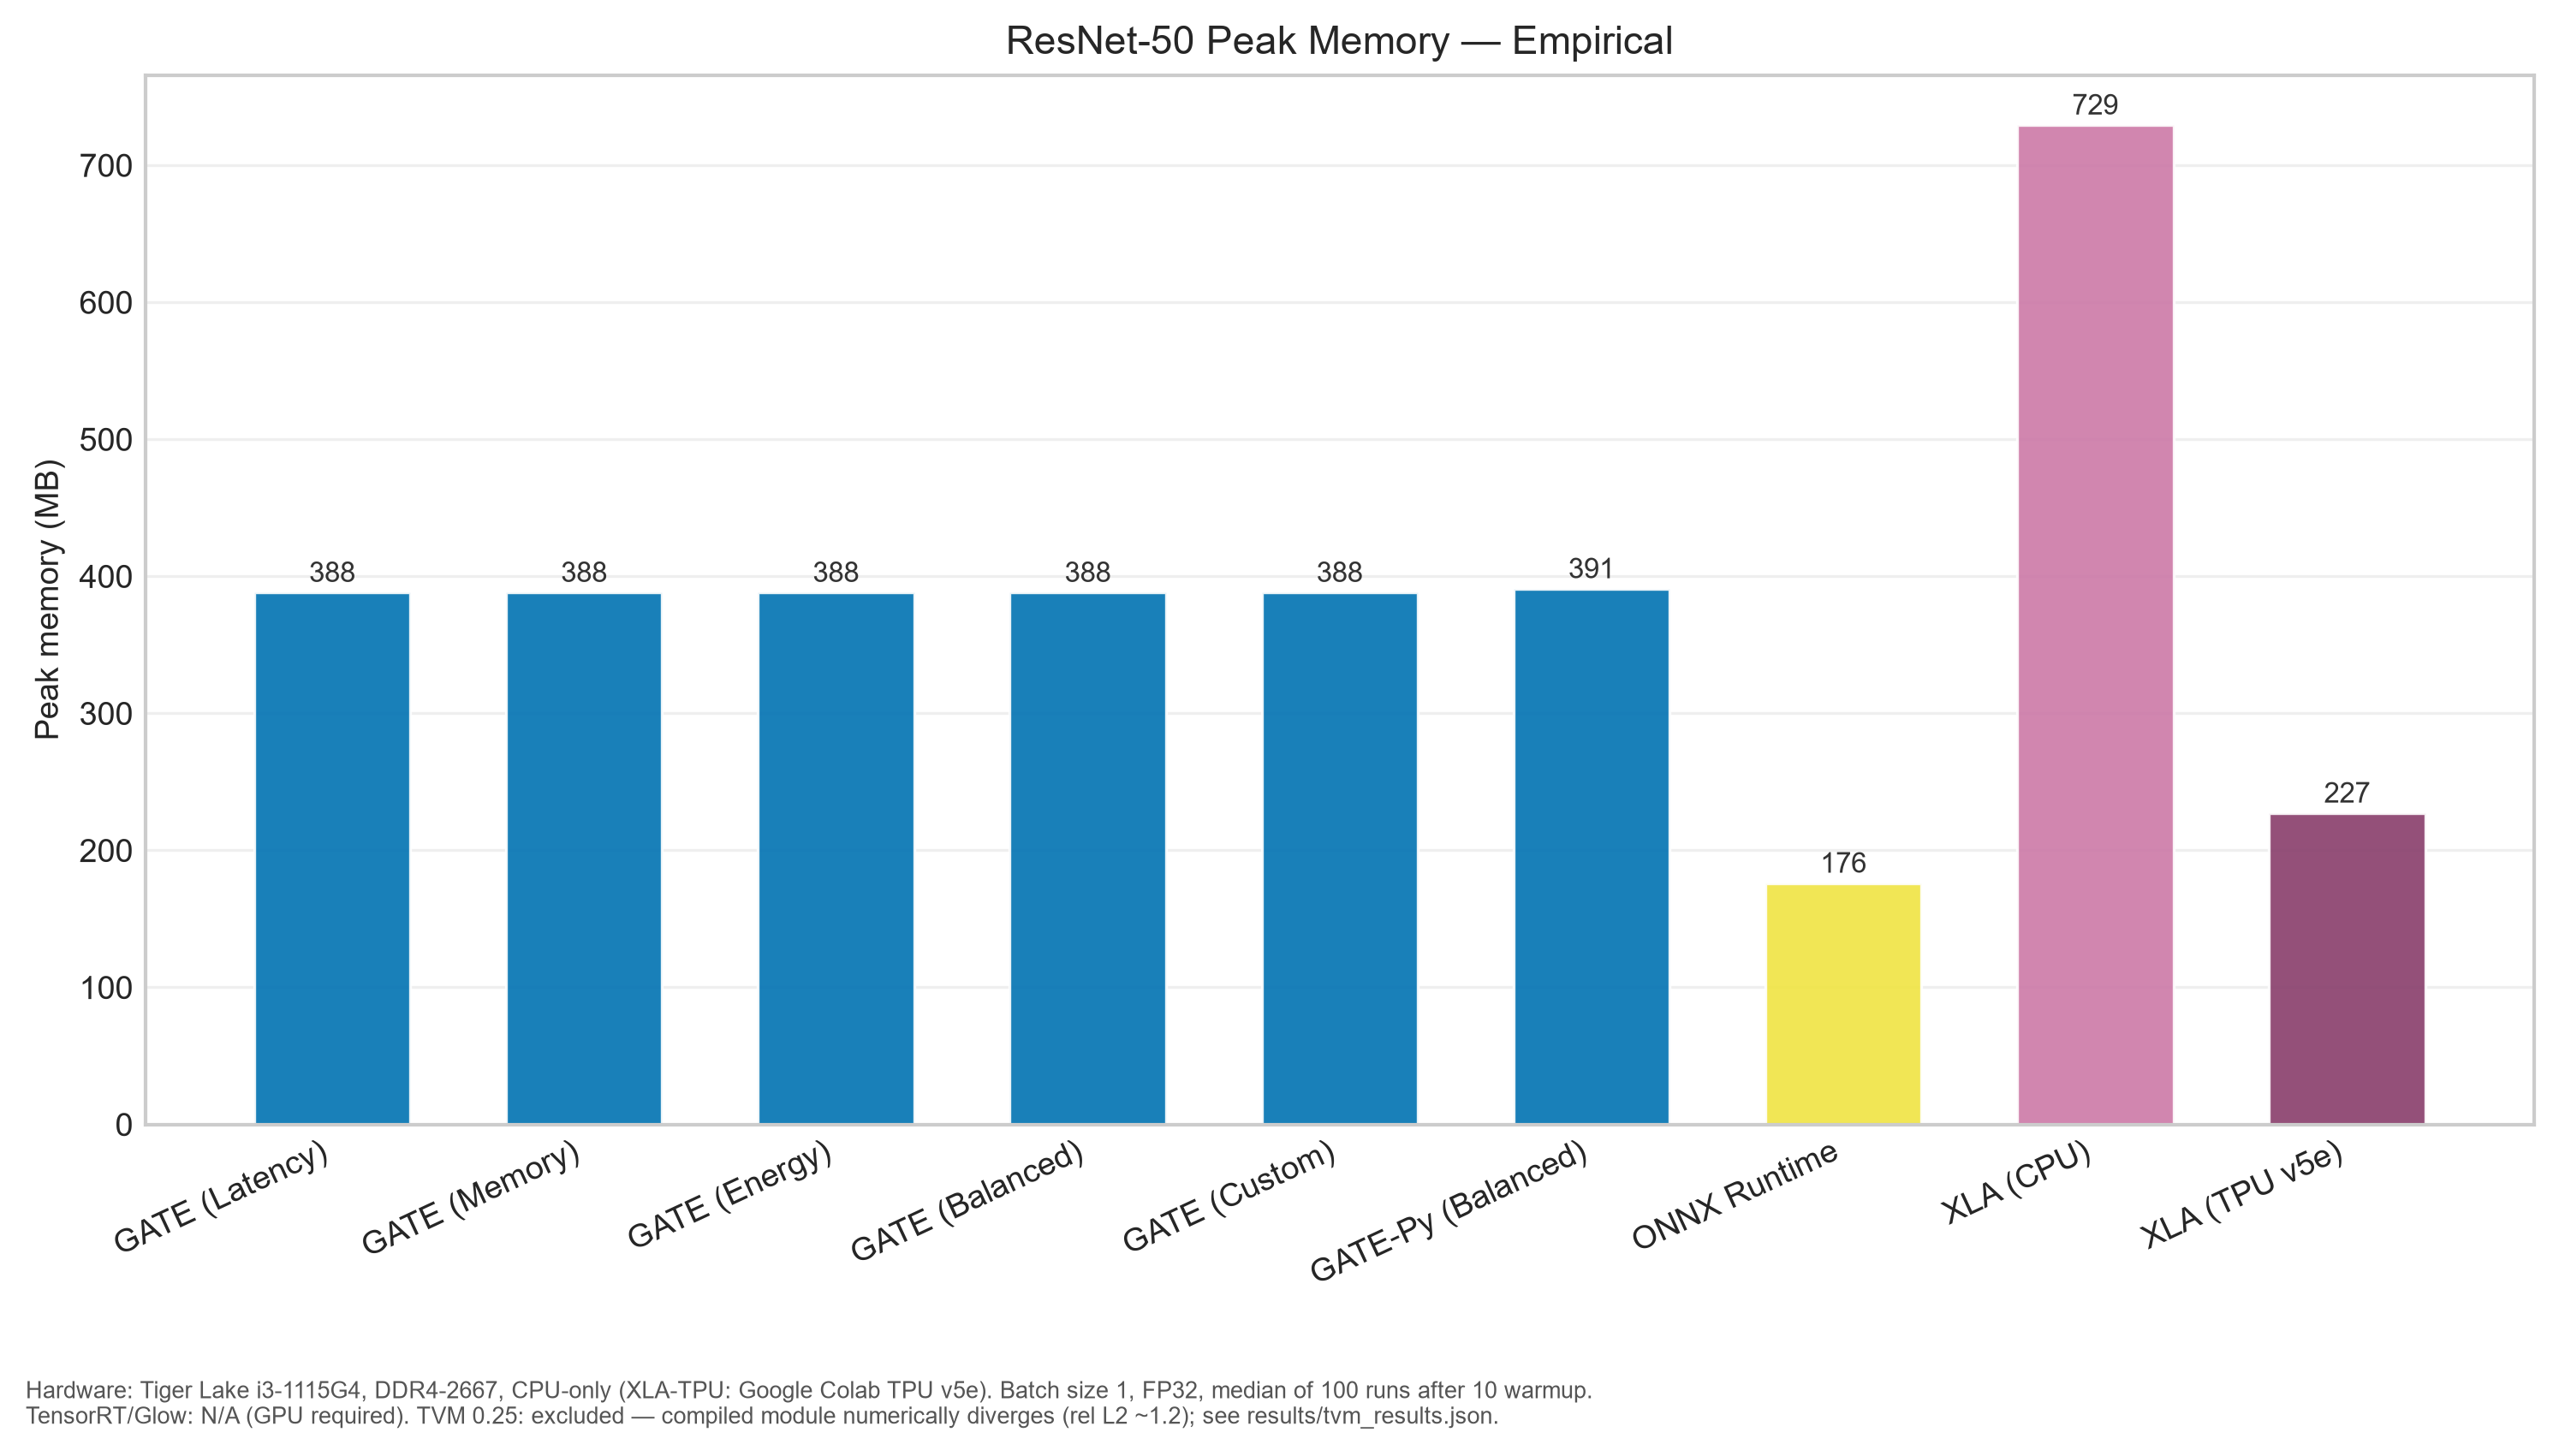
\includegraphics[width=\textwidth]{figures/fig_empirical_memory.png}
    \caption{Peak memory.}
  \end{subfigure}\\[0.6em]
  \begin{subfigure}[t]{0.48\textwidth}
    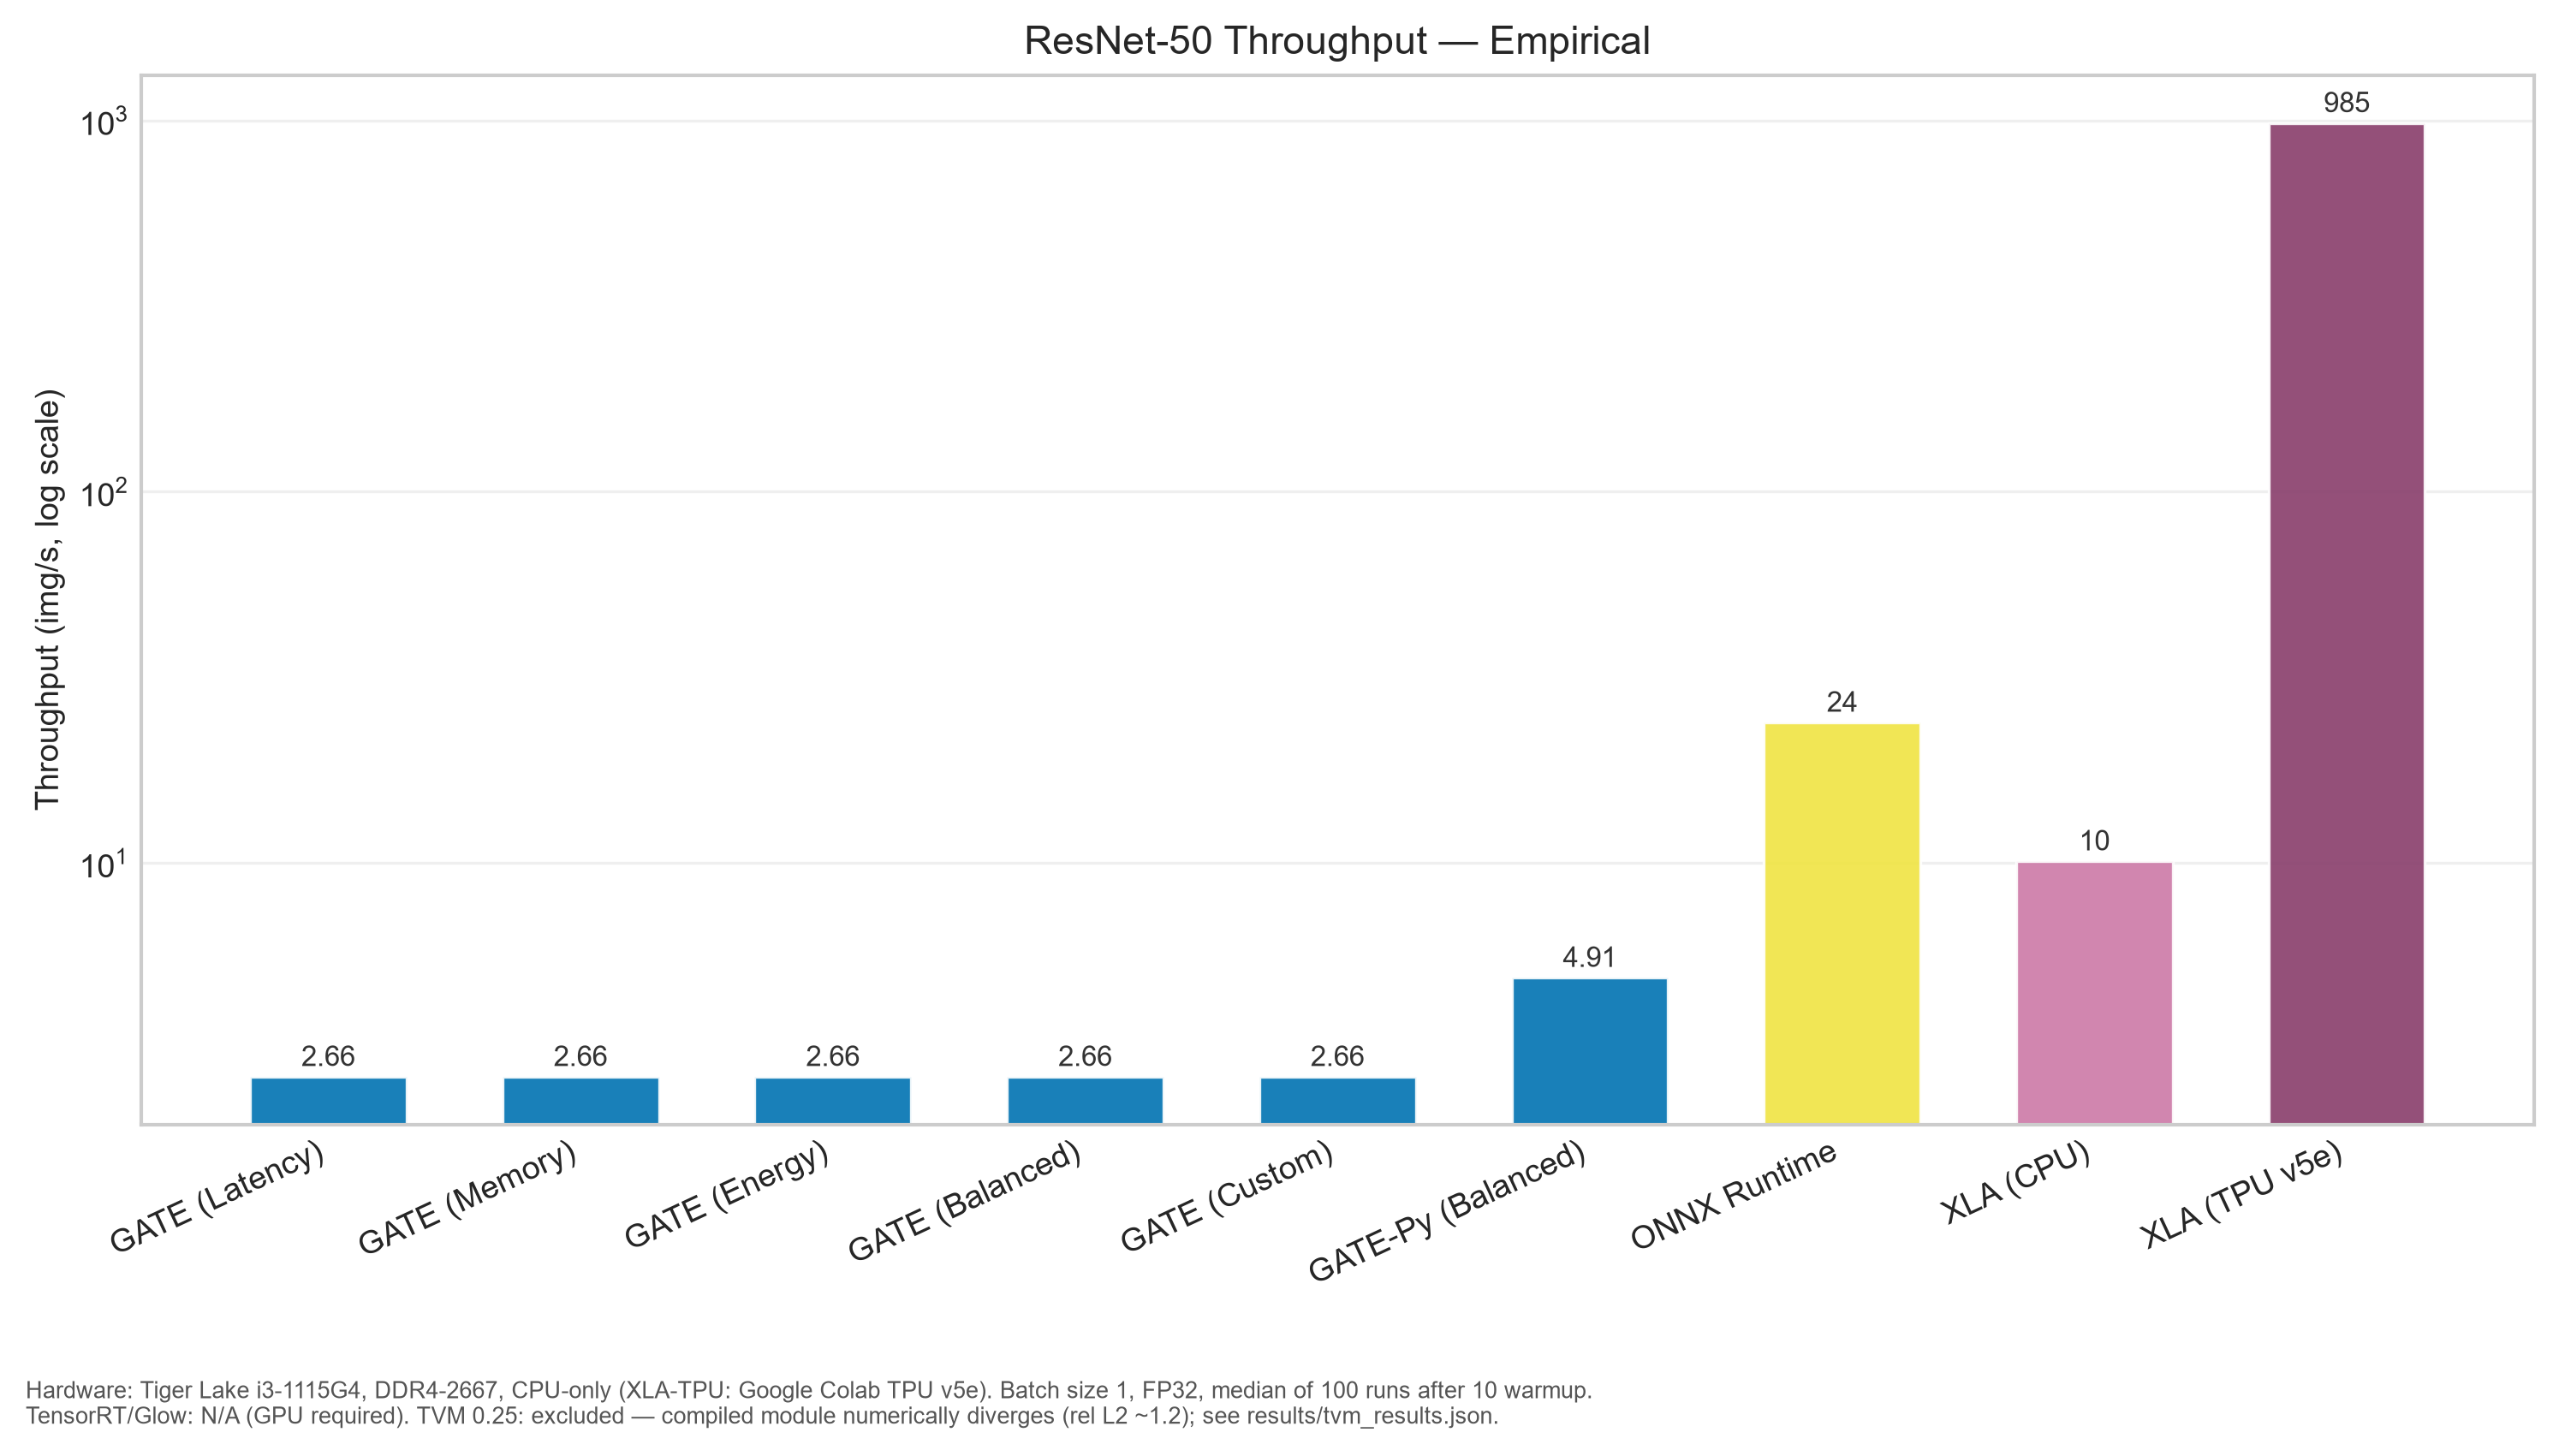
\includegraphics[width=\textwidth]{figures/fig_empirical_throughput.png}
    \caption{Throughput (log scale).}
  \end{subfigure}\hfill
  \begin{subfigure}[t]{0.48\textwidth}
    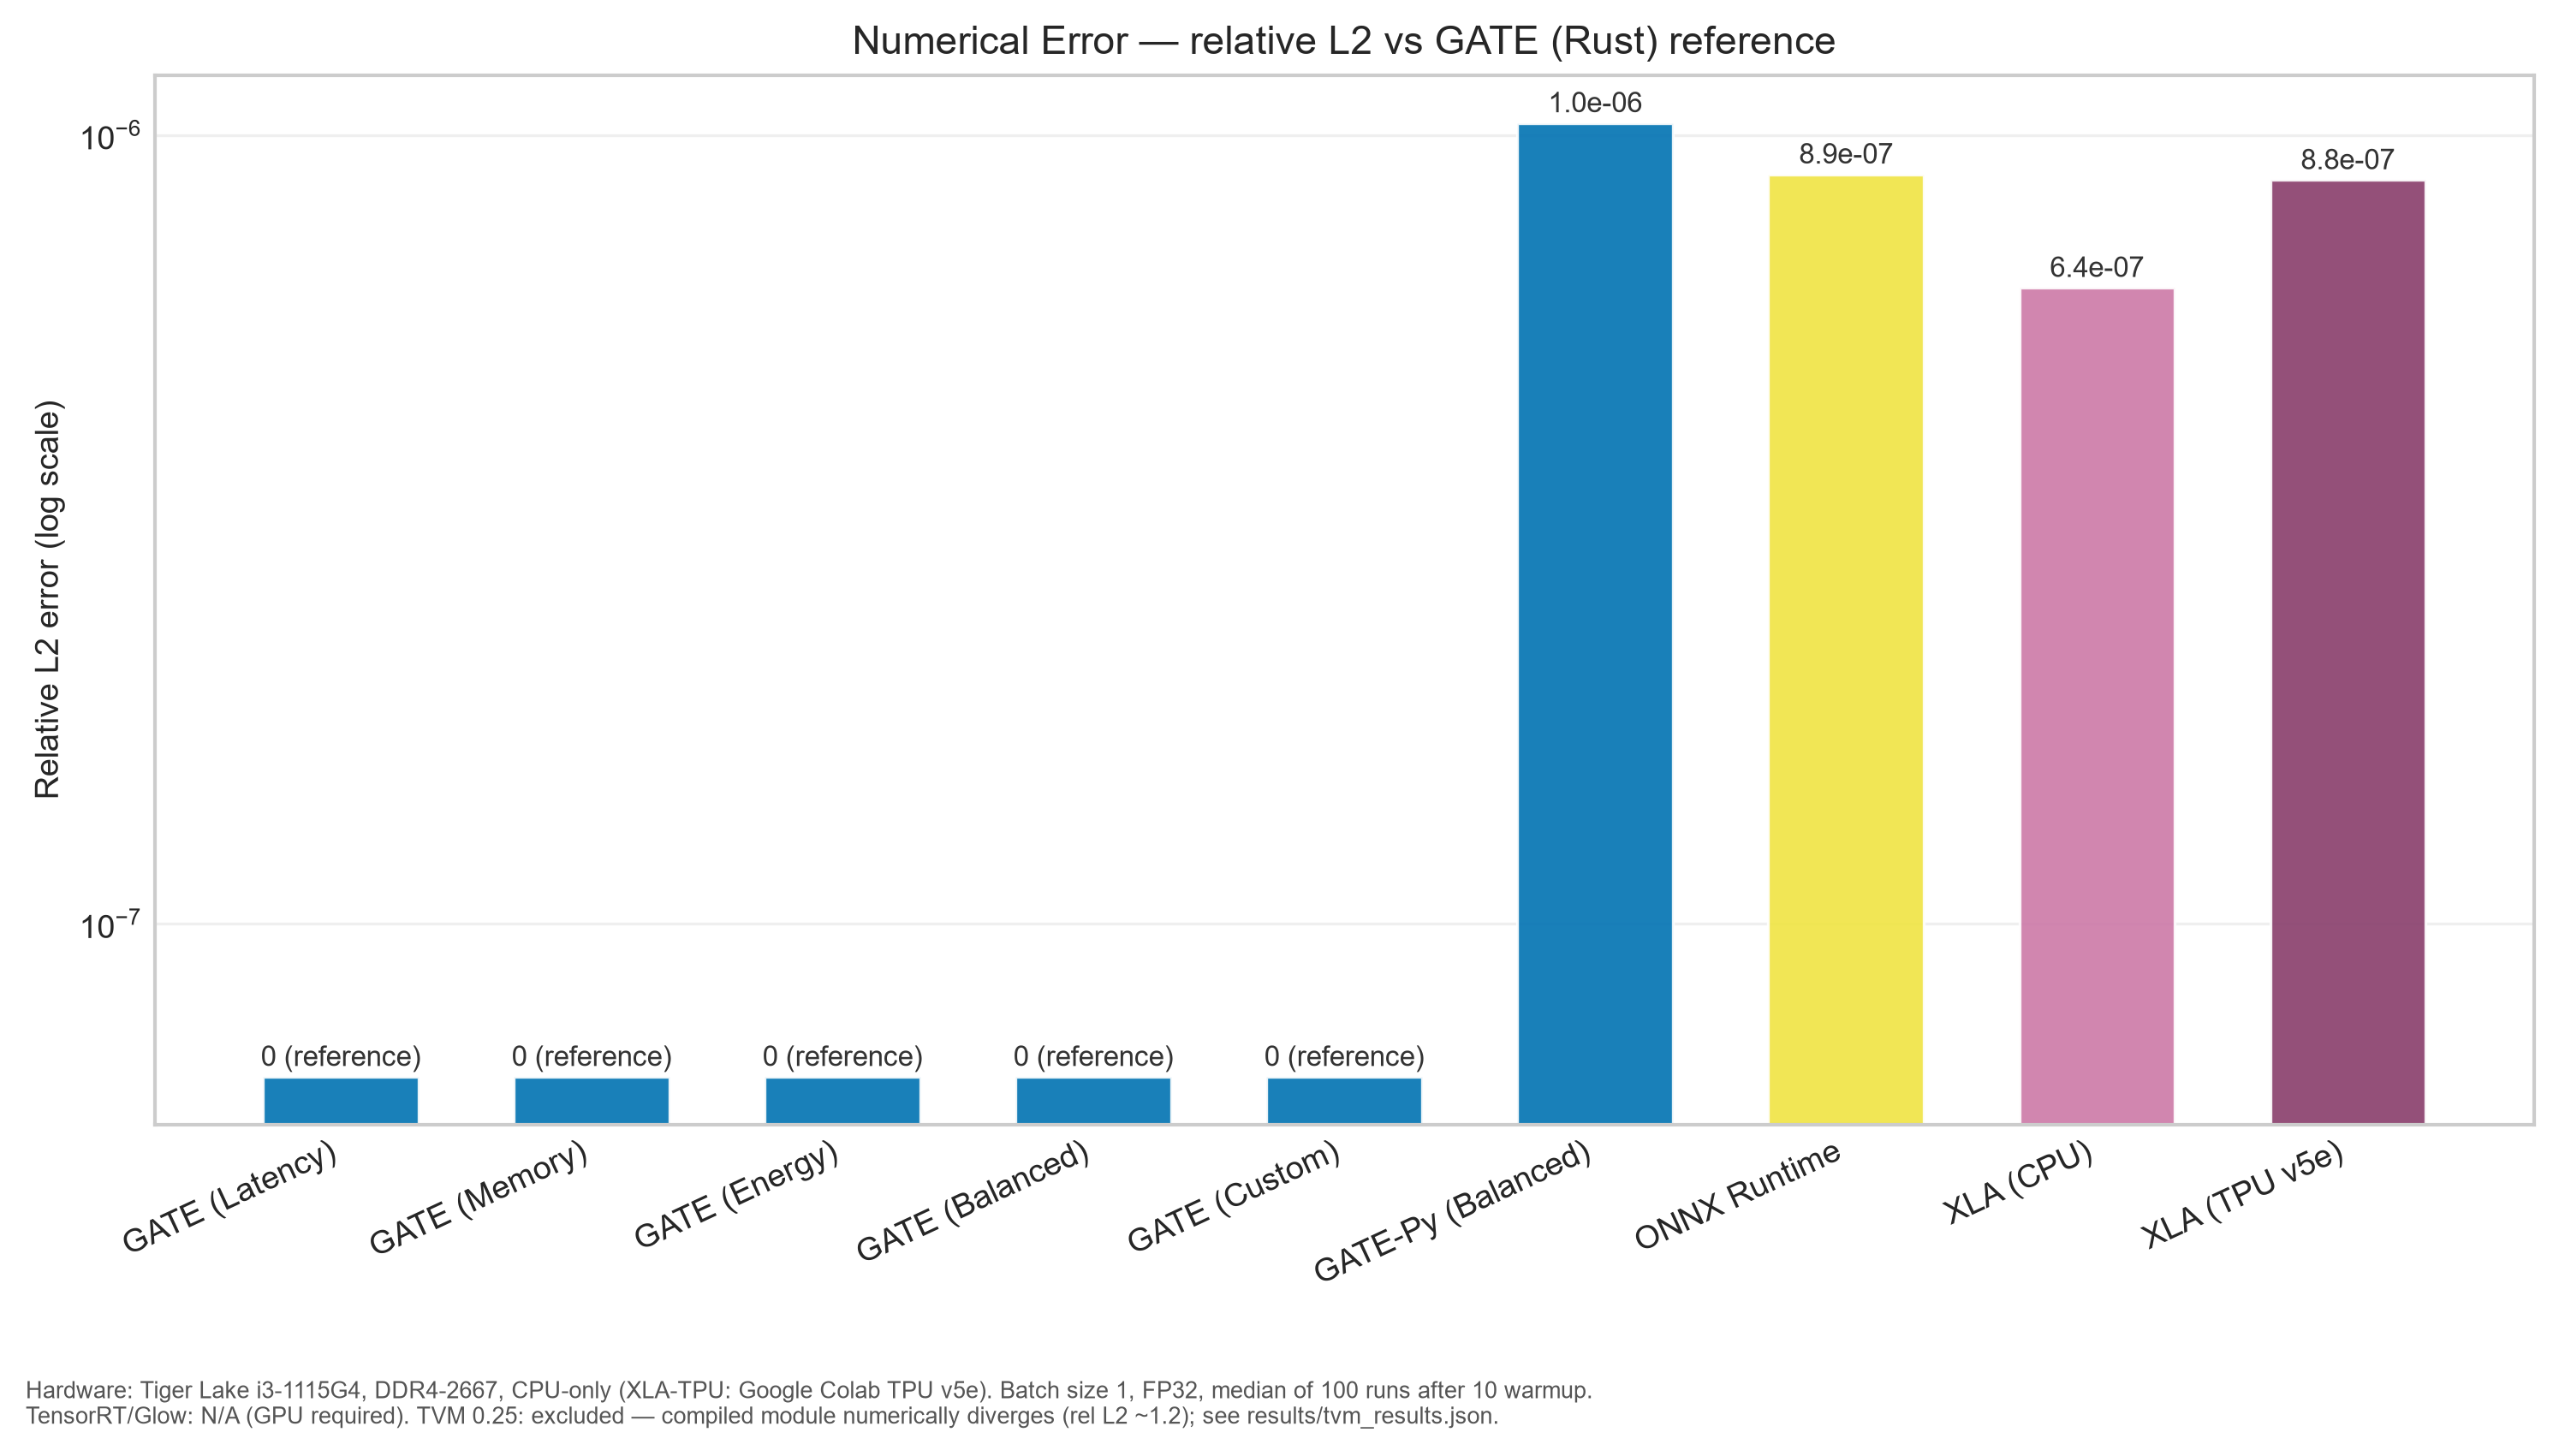
\includegraphics[width=\textwidth]{figures/fig_empirical_numerical_error.png}
    \caption{Numerical error $m_5$ vs.\ \gate{}-Rust.}
  \end{subfigure}
  \caption{Empirical results, ResNet-50, batch 1, FP32, Tiger Lake
  i3-1115G4 (XLA-TPU: Colab TPU v5e).}
  \label{fig:empirical}
\end{figure}

\paragraph{Finding 1: constraint validation is empirically free.}
For $n = 6$ candidates and the full $k = 7$ constraint set, validation
plus cost-minimal selection completes in $1.4$--$8.2\,\mu$s per
policy---seven orders of magnitude below a single inference
(376\,ms)---consistent with the $O(knp)$ bound of
Section~\ref{sec:complexity}. Planning cost is dominated not by the
algorithm but by candidate \emph{calibration} (one real run per
candidate, 6.9\,s total), a one-time cost that amortizes over any
realistic deployment.

\paragraph{Finding 2: the selection criterion is observably
correctness-first.}
On the Latency policy, \gate{} selected the exact plan \texttt{t4}
(4 threads, unfolded BatchNorm) over the ${\sim}6\%$ faster
\texttt{t4\_bnfold}: folding perturbs the output by relative $L_2$ of
$1.1 \times 10^{-6}$, and under max-normalized metrics this nonzero
$m_5$ outweighs the latency gain. \gate{}-Py, whose candidate family
normalizes differently, accepts folding. Both behaviors follow
Theorem~\ref{thm:optimality}---the cost-minimal \emph{valid} plan is
selected---and illustrate how the weight vector, not ad-hoc
heuristics, arbitrates the performance-vs-exactness frontier (see also
Section~\ref{sec:cost}).

\paragraph{Finding 3: a production compiler failed the very constraint
\gate{} enforces.}
TVM 0.25.0 (official win\_amd64 wheel) compiles our ResNet-50 into a
module whose output diverges from all other implementations by
relative $L_2$ of $1.24$--$4.03$ with a \emph{different top-1 class},
despite every per-operator micro-test passing at ${\sim}10^{-7}$. We
isolated a minimal reproduction: any graph containing more than one
\texttt{BatchNormalization} node is lowered incorrectly, while the
imported Relax IR remains correct. Under \gate{}'s protocol such a
plan is rejected by the numerical-error constraint before dispatch;
under TVM's own pipeline it executes silently. We therefore report no
latency for the miscompiled module. This incident is precisely the
failure mode that motivates validating plans \emph{before} optimizing
over them (Section~\ref{sec:design})---and it occurred in an
off-the-shelf release of a widely deployed compiler.

\paragraph{Scope and threats to validity.}
The Rust reference prioritizes auditability over speed (no BLAS, no
intrinsics); its absolute latency is not competitive with production
engines on CPU and we claim no such thing---ONNX Runtime remains
$9\times$ faster on this machine. The TPU~v5e number runs the same JAX
program as the CPU XLA baseline with FP32 matmul precision forced
(\texttt{jax\_default\_matmul\_precision = highest}); it chiefly
demonstrates that the shared-input methodology and the $m_5$ metric
transfer unchanged across a $370\times$ hardware gap. Energy ($m_4$)
on CPU is an analytical estimate (15\,W sustained package power
$\times$ latency; RAPL counters are not exposed on this Windows
platform), and TPU energy is not measurable from a Colab guest. One
machine, one model, batch size 1: these results are a proof-of-concept
companion to---not a replacement for---the analytical study above.
